\documentclass[UTF8]{ctexart}
\CTEXsetup[format={\Large\bfseries}]{section}%默认一级标题居左
\usepackage{geometry}
\geometry{left=2.5cm,right=2.5cm,top=2.5cm,bottom=2.5cm} %页边距
\usepackage{graphicx}%图形
\usepackage{fancyhdr}%页眉页脚
\pagestyle{fancy}	%启用fancy风格设置
\lhead{}
\chead{}
\rhead{\bfseries\textsl{\today}  } % textsl 斜体
\lfoot{}
\cfoot{\thepage}
\rfoot{}
%\renewcommand{\headrulewidth}{0.6pt}    %单线页眉的设置 
\renewcommand{\footrulewidth}{0.4pt}     %单线页脚的设置 
%-----------双线页眉的设置  
\makeatletter % 进入“内部命令模式”(允许使用 @ 符号的 LaTeX 内部变量)
\def\headrule{{\if@fancyplain\let\headrulewidth\plainheadrulewidth\fi%
		\hrule\@height 1.0pt \@width\headwidth\vskip1pt%上面线为1pt粗  
		\hrule\@height 0.5pt\@width\headwidth  %下面0.5pt粗            
		\vskip-2\headrulewidth\vskip-4pt}      %两条线的距离1pt        
		  \vspace{3mm}}     %双线与下面正文之间的垂直间距 
\makeatother    % 退出“内部命令模式”
%------------双线页眉的设置            
% \usepackage{booktabs}
% \usepackage{subfigure}
\usepackage{setspace}
\usepackage{amsmath}
\usepackage{array}%需要该宏包
\usepackage{diagbox} % 加载宏包
\usepackage{multirow}
\usepackage{textcomp}
\usepackage{indentfirst}%首行缩进宏包
\usepackage{setspace}
\usepackage{amssymb}
\usepackage{listings}
\usepackage{xcolor}    % 可选:代码着色(示例用)
\lstset{
    frame = single,                % 添加边框(single 表示单线边框)
    numbers = left,                % 在左侧显示行号
    numberstyle = \tiny\color{gray}, % 行号样式
    basicstyle = \ttfamily,        % 设置等宽字体
    keywordstyle = \color{blue},    % 关键字颜色
    commentstyle = \color{green},   % 注释颜色
    stringstyle = \color{red},      % 字符串颜色
    breaklines = true,             % 自动换行
    showstringspaces = false,      % 不显示字符串中的空格
    tabsize = 4                    % 设置缩进空格数
}
\usepackage[colorlinks=true,pdfborder={0 0 0},
    linkcolor=red,     % 内部链接(如目录→章节)的文字颜色
    citecolor=green,    % 引用(如\cite)的文字颜色
    urlcolor=blue,      % 网址的文字颜色
]{hyperref} %超链接
\usepackage{float}  % 提供 [H] 选项

\title{{\heiti  第四周实验:调试与性能分析、元编程、pytorch }\vspace{-2em}}
\date{}
\begin{document}
\thispagestyle{empty}  %用于设置 “当前页” 的页眉页脚风格:
\begin{figure}[tph!] %封面标题
	\centering
	
\includegraphics[width=0.7\linewidth]{figure/2}
	
\end{figure}

\begin{center}% % 内容居中环境(所有内部内容均居中对齐)
	\quad \\ %插入一个小空格
	\quad \\
	\quad \\
	\quad \\
	% \quad \\
	% \quad \\
	\heiti \fontsize{30}{17} \quad \quad 第\quad 四\quad 周\quad \quad \quad 
	\vskip 0.5cm
	\songti \zihao{2} 实\quad 验\quad 报\quad 告%在此打印论文题目,二号黑体	
\end{center}
\vskip 1cm

\begin{quotation}
	\songti \fontsize{20}{20}
	\doublespacing
	\par\setlength\parindent{12em}
	\qquad
\begin{center}
		{\Large 学\hspace{0.88cm} 院:\underline{\hbox to 58mm{信息科学与工程学部\hfill}}}
		\vskip 0.3cm	
		{\Large 班\hspace{0.88cm} 号:\underline{\hbox to 58mm{计科一班\hfill}}}
		\vskip 0.3cm
		{\Large 姓\hspace{0.88cm} 名:\underline{\hbox to 58mm{顾晓宁\hfill}}}
		\vskip 0.3cm	
		{\Large 学\hspace{0.88cm} 号:\underline{\hbox to 58mm{24020007036\hfill}}}
		\vskip 0.3cm	
		{\Large 实验编号:\underline{\hbox to 58mm{第四周实验报告\hfill}}}
		\vskip 0.3cm	
		{\Large 指导教师:\underline{\hbox to 58mm{周小伟\hfill}}}
	\end{center}
	% \vskip 3cm
	% \begin{flushright}% 日期右对齐
	% 	% 2019\;年\;5\;月\;14\;日
	% 	\today
	% \end{flushright}
	
\end{quotation}
\newpage
%\thispagestyle{empty}
\tableofcontents % 自动生成目录(基于后续的 \section、\subsection 等章节命令)
\newpage
\maketitle	
\thispagestyle{fancy}	
\section{实验目的}
\textbf{初试调试与性能分析,元编程,以及pytorch}
\section{练习内容与结果}
\subsection{调式与性能分析}
\subsubsection{获取最近一天中超级用户的登录信息及其所执行的指令。如果找不到相关信息,您可以执行一些无害的命令,例如 sudo ls 然后再次查看。}
Linux可以使用journalctl,macOS可以使用log show。
\begin{lstlisting}
	journalctl --since "2025-09-15 00:00:00" --until "2025-09-15 23:59:59" | grep "sudo"
\end{lstlisting}
\begin{figure}[H]
	\centering
	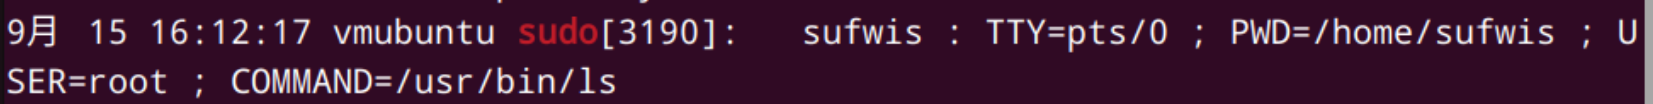
\includegraphics[width=0.7\linewidth]{figure/journal.png}
	\caption{如图,sudo用户执行过ls操作}
\end{figure}

\subsubsection{安装 shellcheck 并尝试对下面的脚本进行检查。这段代码有什么问题吗?请修复相关问题。}
\begin{lstlisting}
	#!/bin/sh
	## Example: a typical script with several problems
	for f in $(ls *.m3u)
	do
	grep -qi hq.*mp3 $f \
		&& echo -e 'Playlist $f contains a HQ file in mp3 format'
	done
\end{lstlisting}
\indent	配置好ALE和shellcheck后,如图所示,淡红色背景色标注错误处,同时移动到每行错误代码时会提示错误信息。
\begin{figure}[H]
	\centering
	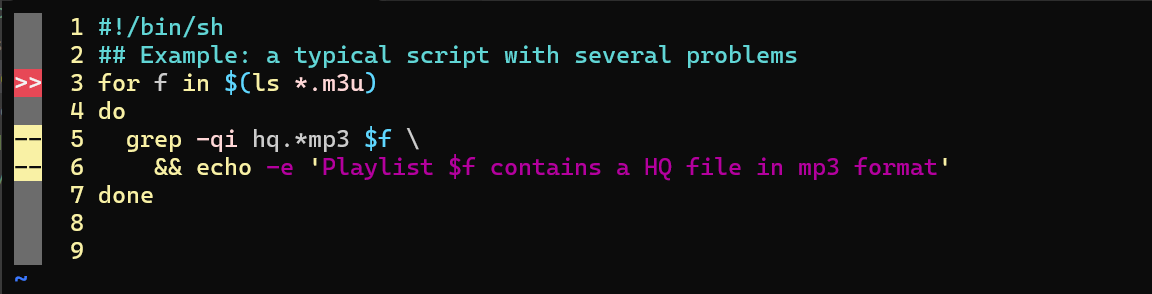
\includegraphics[width=0.7\linewidth]{figure/shellcheck.png}
	\caption{如图}
\end{figure}


\subsubsection{gdb:启动与退出}
使用gcc为例。
\\
\indent 使用gcc编译时,使用-g参数
\begin{verbatim}
	启动gdb
	$ gdb 可执行程序
	命令行传参
	# 设置的时机: 启动gdb之后, 在应用程序启动之前
	(gdb) set args 参数1 参数2 .... ...
	# 查看设置的命令行参数
	(gdb) show args

	对应的命令行参数为main函数的
	int argc, char* argv[]
	argc命令数量
	argv[0]是程序名,argv[1]及以后是传递的参数

	run: 可以缩写为 r, 如果程序中设置了断点会停在第一个断点的位置, 
		如果没有设置断点, 程序就执行完了
	start: 启动程序, 最终会阻塞在main函数的第一行,等待输入后续其它 gdb 指令
	continue: 如果想让程序start之后继续运行, 
		或者在断点处继续运行,可以使用 continue命令, 可以简写为 c

	退出gdb
	# quit == q
	(gdb) quit
\end{verbatim}

\subsubsection{gdb:查看代码}
\begin{verbatim}
	list 从第一行开始现实
	list 行号
	list 函数名
	默认十行
	默认初始文件是main所在的文件
	
	# 切换到指定的文件,并列出这行号对应的上下文代码, 默认情况下只显示10行内容
	(gdb) l 文件名:行号

	# 切换到指定的文件,并显示这个函数的上下文内容, 默认显示10行
	(gdb) l 文件名:函数名

	# 以下两个命令中的 listsize 都可以写成 list
	(gdb) set listsize 行数

	# 查看当前list一次显示的行数
	(gdb) show listsize
\end{verbatim}

\subsubsection{gdb:断点设置}
\begin{verbatim}
	当前文件普通断点
	# 在当前文件的某一行上设置断点
	# break == b
	(gdb) b 行号
	(gdb) b 函数名		# 停止在函数的第一行

	普通断点非当前文件
	# 在非当前文件的某一行上设置断点
	(gdb) b 文件名:行号
	(gdb) b 文件名:函数名		# 停止在函数的第一行

	条件断点
	# 必须要满足某个条件, 程序才会停在这个断点的位置上
	# 通常情况下, 在循环中条件断点用的比较多
	(gdb) b 行数 if 条件
\end{verbatim}



\subsubsection{gdb:断点操作}
\begin{verbatim}
	info break命令查看设置的断点信息,其中info可以缩写为i
	(gdb) i b   #info break
	断点信息:
	Num: 断点的编号, 删除断点或者设置断点状态的时候都需要使用
	Enb: 当前断点的状态, y表示断点可用, n表示断点不可用
	What: 描述断点被设置在了哪个文件的哪一行或者哪个函数上

	删除:
	d 断点编号
	d 断点编号1-断点编号2 // 范围删除

	设置状态:
	禁用
	dis/disable 断点编号
	dis/disable 断点编号1-断点编号2
	启用
	ena/enable 断点编号
	ena/enable 断点编号1-断点编号2
\end{verbatim}

\subsubsection{gdb:打印信息}
\begin{verbatim}
	# print == p
	# 分别对应值、类型
	(gdb) p 变量名
	(gdb) ptype 变量名

	# 如果变量是一个整形, 默认对应的值是以10进制格式输出, 其他格式请参考上表
	(gdb) p/fmt 变量名
	/fmt格式如下:
	格式化字符(/fmt)	说明
	/x	以十六进制的形式打印出整数。
	/d	以有符号、十进制的形式打印出整数。
	/u	以无符号、十进制的形式打印出整数。
	/o	以八进制的形式打印出整数。
	/t	以二进制的形式打印出整数。
	/f	以浮点数的形式打印变量或表达式的值。
	/c	以字符形式打印变量或表达式的值。
\end{verbatim}

\subsubsection{gdb:自动打印信息}
\begin{verbatim}
	(gdb) display 变量名
	(gdb) display/fmt 变量名
	/fmt 同上
\end{verbatim}

\subsubsection{gdb:显示自动打印变量表}
\begin{verbatim}
	i/info display
	
	Num : 变量或表达式的编号,GDB 调试器为每个变量或表达式都分配有唯一的编号
	Enb : 表示当前变量(表达式)是处于激活状态还是禁用状态,
		如果处于激活状态(用 y 表示),则每次程序停止执行,该变量的值都会被打印出来;
		反之,如果处于禁用状态(用 n 表示),则该变量(表达式)的值不会被打印。
	Expression :被自动打印值的变量或表达式的名字。
\end{verbatim}

\subsubsection{gdb:自动打印变量的删除、禁用和启用}
\begin{verbatim}
	(gdb) delete display num [num1 ...]
	(gdb) delete display num1-numN
	
	禁用和启用:
	分别对应dis,ena
\end{verbatim}



\subsection{元编程}
\subsubsection{make:基础语法}
Makefile的框架是由规则构成的。make命令执行时先在Makefile文件中查找各种规则,对各种规则进行解析后运行规则。
\\
\indent 规则的基本格式为:
\begin{verbatim}
	target1,target2...: depend1, depend2, ...
		command
		......
		......
	目标(target), 依赖(depend)和命令(command)	
	命令(command): 当前这条规则的动作,一般情况下这个动作就是一个 shell 命令
	依赖(depend): 规则所必需的依赖条件,在规则的命令中可以使用这些依赖。
	目标(target): 规则中的目标,这个目标和规则中的命令是对应的
\end{verbatim}

\subsubsection{make:规则的执行}
在调用 make 命令编译程序的时候,make 会首先找到 Makefile 文件中的第 1 个规则,分析并执行相关的动作。
可以将不存在的依赖作为新的规则中的目标,当这条新的规则对应的命令执行完毕,对应的目标就被生成了,同时另一条规则中需要的依赖也就存在了。
\\
\indent 单独执行规则:
make target。
将单独执行对应target目标后的规则。
\\
\indent 常用的是制作clear伪目标,用于清理中间、目标文件。

\subsubsection{make:按时间戳更新}
目标是通过依赖生成的,因此正常情况下:目标时间戳 > 所有依赖的时间戳, 如果执行 make 命令的时候检测到规则中的目标和依赖满足这个条件, 那么规则中的命令就不会被执行。
\\
\indent 当依赖文件被更新了, 文件时间戳也会随之被更新, 这时候 目标时间戳 < 某些依赖的时间戳, 在这种情况下目标文件会通过规则中的命令被重新生成。
\\
\indent	如果规则中的目标对应的文件根本就不存在, 那么规则中的命令肯定会被执行。

\subsubsection{make:自动推导}
因为 make 有自动推导的能力,不会完全依赖 makefile。
\begin{verbatim}
	# 这是一个完整的 makefile 文件
		calc:add.o  div.o  main.o  mult.o  sub.o
        gcc  add.o  div.o  main.o  mult.o  sub.o -o calc
\end{verbatim}
注意:\\
\indent 依赖中所有的 .o文件在本地项目目录中是不存在的, 并且也没有其他的规则用来生成这些依赖文件, 这时候 make 会使用内部默认的构造规则先将这些依赖文件生成出来。

\subsubsection{make:变量}
\begin{itemize}
	\item 自定义变量
	\item 预定义变量
	\item 自动变量
\end{itemize}
自定义变量:
\begin{verbatim}
	定义:
	变量名=变量值
	获取:
	$(变量的名字)
\end{verbatim}
预定义变量:
\begin{verbatim}
	AR			生成静态库库文件的程序名称	ar
	AS			汇编编译器的名称			as
	CC			C 语言编译器的名称			cc
	CPP			C 语言预编译器的名称		$(CC) -E
	CXX			C++语言编译器的名称	 		g++
	ARFLAGS		生成静态库库文件程序的选项	无默认值
	ASFLAGS		汇编语言编译器的编译选项	无默认值
	CFLAGS		C 语言编译器的编译选项		无默认值
	CPPFLAGS	C 语言预编译的编译选项		无默认值
	CXXFLAGS	C++语言编译器的编译选项		无默认值
\end{verbatim}
自动变量(规则中的目标文件和依赖文件,并且它们只能在规则的命令中使用):
\begin{verbatim}
	$*	表示目标文件的名称,不包含目标文件的扩展名
	$+	表示所有的依赖文件,这些依赖文件之间以空格分开,按照出现的先后为顺序,其中可能 包含重复的依赖文件
	$<	表示依赖项中第一个依赖文件的名称
	$?	依赖项中,所有比目标文件时间戳晚的依赖文件,依赖文件之间以空格分开
	$@	表示目标文件的名称,包含文件扩展名
	$^	依赖项中,所有不重复的依赖文件,这些文件之间以空格分开
\end{verbatim}


\subsubsection{make:模式匹配}
将.c文件编译为.o目标文件,使用自动变量,因为依赖项不固定。
\begin{verbatim}
	# 模式匹配 -> 通过一个公式, 代表若干个满足条件的规则
	# 依赖有一个, 后缀为.c, 生成的目标是一个 .o 的文件, % 是一个通配符, 匹配的是文件名
	%.o:%.c
		gcc $< -c
\end{verbatim}

\subsubsection{make:函数}
\begin{verbatim}
	函数调用
	$(函数名 参数1, 参数2, 参数3, ...)
	函数定义
	define function_name
	# 函数体
	# 可以使用 $(1), $(2), $(3)... 来引用第1、2、3...个参数
	# 可以使用 $(0) 来引用函数名本身
	endef
	自定义函数调用
	$(call function_name,argument1,argument2,...)
\end{verbatim}
常用函数:
\begin{verbatim}
	# 该函数的参数只有一个, 但是这个参数可以分成若干个部分, 通过空格间隔
	参数:	指定某个目录, 搜索这个路径下指定类型的文件,比如: *.c
	$(wildcard PATTERN...)

	# 有三个参数, 参数之间使用 逗号间隔
	$(patsubst <pattern>,<replacement>,<text>)
	pattern:要替换的文件和后缀,使用通配符,如%.c
	replacement :替换后的,如%.o
	text:要替换的字符串
	返回值:替换后的字符串
\end{verbatim}


\subsubsection{make:示例}
\begin{lstlisting}
	src=$(wildcard *.c)
	obj=$(patsubst %.c, %.o, $(src))
	target=calc

	$(target):$(obj)
			gcc $(obj)  -o $(target)

	%.o:%.c
			gcc $< -c

	.PHONY:clean
	clean:
        	-rm $(obj) $(target) 		
\end{lstlisting}


\subsection{pytorch}
\begin{verbatim}
	使用pytorch制作一个简单的ai,配合该目录下CNN_test.py食用更加。
\end{verbatim}

\subsubsection{数据集}
\begin{verbatim}
	导入必要的库
	import torch
	import torch.nn as nn
	import torch.nn.functional as F
	import torch.optim as optim
	from torchvision import datasets, transforms
	device设置,如果支持cuda,可以将运算移动至GPU上:
	device = torch.device('cuda' if torch.cuda.is_available() else 'cpu')

	# 1. 数据加载与预处理
	transform = transforms.Compose([
		transforms.ToTensor(),  # 转为张量
		transforms.Normalize((0.5,), (0.5,))  # 归一化到 [-1, 1],
		# 处理的是灰度图
	])

	# 加载 MNIST 数据集
	train_dataset = datasets.MNIST(root='./data', train=True, transform=transform, download=True)
	test_dataset = datasets.MNIST(root='./data', train=False, transform=transform, download=True)

	# 定义加载器
	train_loader = torch.utils.data.DataLoader(dataset=train_dataset, batch_size=64, shuffle=True)
	test_loader = torch.utils.data.DataLoader(dataset=test_dataset, batch_size=64, shuffle=False)

\end{verbatim}


\subsubsection{模型}
\begin{verbatim}
	class SimpleCNN(nn.Module):
		def __init__(self):
			super(SimpleCNN, self).__init__()
			# 定义卷积层
			# 输出尺寸=(输入尺寸-kernel_size+2*padding)/stride + 1
			self.conv1 = nn.Conv2d(1, 32, kernel_size=3, stride=1, padding=1)  # 输入1通道,输出32通道
			self.conv2 = nn.Conv2d(32, 64, kernel_size=3, stride=1, padding=1)  # 输入32通道,输出64通道
			# 定义全连接层
			self.fc1 = nn.Linear(64 * 7 * 7, 128)  # 展平后输入到全连接层
			self.fc2 = nn.Linear(128, 10)  # 10 个类别

		def forward(self, x):
			x = F.relu(self.conv1(x))  # 第一层卷积 + ReLU
			x = F.max_pool2d(x, 2)     # 最大池化,参数2表示2×2的正方形池化窗口
			x = F.relu(self.conv2(x))  # 第二层卷积 + ReLU
			x = F.max_pool2d(x, 2)     # 最大池化
			x = x.view(-1, 64 * 7 * 7) # 展平
			x = F.relu(self.fc1(x))    # 全连接层 + ReLU
			x = self.fc2(x)            # 最后一层输出
			return x
\end{verbatim}


\subsubsection{训练与测试}
\begin{verbatim}
		
	# 创建模型实例
	model = SimpleCNN().to(device)

	# 3. 定义损失函数与优化器
	criterion = nn.CrossEntropyLoss()  # 多分类交叉熵损失
	optimizer = optim.SGD(model.parameters(), lr=0.01, momentum=0.9)

	# 4. 模型训练
	num_epochs = 10
	model.train()  # 设置模型为训练模式

	for epoch in range(num_epochs):
		total_loss = 0
		for images, labels in train_loader:
			images=images.to(device)
			labels=labels.to(device)

			outputs = model(images)  # 前向传播
			loss = criterion(outputs, labels)  # 计算损失

			optimizer.zero_grad()  # 清空梯度
			loss.backward()  # 反向传播
			optimizer.step()  # 更新参数

			total_loss += loss.item()

		print(f"Epoch [{epoch+1}/{num_epochs}], Loss: {total_loss / len(train_loader):.4f}")

	# 5. 模型测试
	model.eval()  # 设置模型为评估模式
	correct = 0
	total = 0

	with torch.no_grad():  # 关闭梯度计算
		for images, labels in test_loader:
			images = images.to(device)
			labels = labels.to(device)
			outputs = model(images)
			_, predicted = torch.max(outputs, 1)
			total += labels.size(0)
			correct += (predicted == labels).sum().item()

	accuracy = 100 * correct / total
	print(f"Test Accuracy: {accuracy:.2f}%")

	torch.save(model.state_dict(),"pytorch-basic-other\\CNN_test_model_statedict.pth")
\end{verbatim}


\section{实验感悟}
调试和性能分析工具,建议在有对应需求时,熟练掌握。
pytorch集成了很对有用的模块,使用者甚至不需要理解其内部本质,
只需要了解大概流程,即可训练出自己的AI。


\section{个人github/gitee账号}
\href{https://github.com/sufwis}{个人github账号}\\
\indent \href{https://github.com/sufwis/development-tools-learn.git}{对应仓库}

\section{推荐阅读}
\href{https://missing-semester-cn.github.io/2020/debugging-profiling/}{调试及性能分析}
\\
\indent \href{https://missing-semester-cn.github.io/2020/metaprogramming/}{元编程}
\\
\indent \href{https://www.runoob.com/pytorch/pytorch-tutorial.html}{PyTorch 教程}
\\
\indent \href{https://subingwen.cn/}{make、gdb基础介绍来自:\\\indent \qquad 作者: 苏丙榅\\
\indent \qquad 来源: 爱编程的大丙\\
\indent \qquad 著作权归作者所有。商业转载请联系作者获得授权,非商业转载请注明出处。
}
\end{document}